\section{Einleitung}
\subsection{Motivation}
%
%
\begin{frame}
	\frametitle{Überblick}
	\tableofcontents[currentsubsection]
\end{frame}
%
%
\begin{frame}
	\frametitle{Kleine und große Katastrophen (1)}
	\begin{figure}
		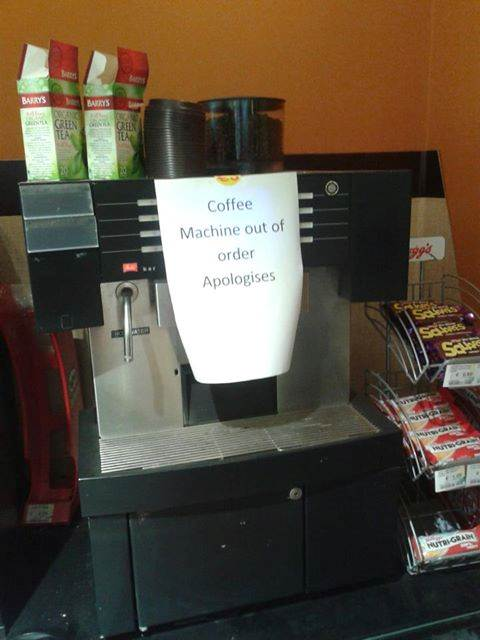
\includegraphics[scale=0.36]{grafiken/broken2}
		
		
	
		
		\caption{Kleine Katastrophe - defekte Kaffeemaschine
			\footnote{\tiny Quelle: \url{https://jlonerga.wordpress.com} }
		}		
	\end{figure}
\end{frame}
%
%
\begin{frame}
	\frametitle{Kleine und große Katastrophen (2)}
	Dreyfus
\end{frame}%
%
\begin{frame}
	\frametitle{Historischer Gedanke}
	Dreyfus
\end{frame}
\begin{frame}
	\frametitle{Redundanz}
	Warum:
	\begin{itemize}
		\item 1 
		\item 2
		\item 2
	\end{itemize}	
	
\end{frame}

\subsection{Redundanz als Ansatz für zuverlässige Systeme}
